\documentclass[10pt,letterpaper]{article}
\usepackage{setspace}
\usepackage{float}
\usepackage[utf8]{inputenc}
\usepackage[top=1in,bottom=1in,right=1.0in,left=1.0in]{geometry}
\usepackage{times}
\usepackage{graphicx}
\usepackage{amsmath,amssymb} % define this before the line numbering.
\usepackage{color}
\usepackage[breaklinks=true,bookmarks=false,colorlinks=true,citecolor=green,urlcolor=blue,linkcolor=black]{hyperref}
\usepackage{booktabs}
\usepackage{epstopdf}
\usepackage{pdfpages}
\usepackage{hyphenat}
\usepackage{fancyhdr}
\usepackage{wrapfig}
\usepackage[font=small,labelfont=bf]{caption}
\usepackage{booktabs}
\usepackage{multirow}
\usepackage{parskip}
\usepackage{enumitem}
\usepackage{hyperref}
\pagenumbering{gobble}

\title{
	\Large{\textbf{Uncertainty-Aware Hybrid Rendering with Gaussian
			Splatting and NeRF for High-Fidelity Synthesis}}
}

\date{\small April 2025}
\author{
	Team 25 Patrick Chen\\
	\small\texttt{bochunc@andrew.cmu.edu}	\\\\
	\large Robotics Institute, School of Computer Science, Carnegie Mellon University
}
\usepackage{lastpage}

\begin{document}
	
	\maketitle
	\thispagestyle{empty}
\section*{Abstract}
\noindent Efficient 3D rendering often involves a trade-off between speed and quality. \textbf{3D Gaussian Splatting (GS)} offers fast rendering but lacks fine detail, while \textbf{NeRF} delivers high fidelity at a high computational cost. We propose an \textbf{uncertainty-aware hybrid rendering framework} that combines the strengths of both, selectively applying NeRF to uncertain regions identified via a lightweight U-Net or MLP predictor trained on GS-derived features. Our best-performing model, \textbf{Hybrid-MLP 50\%}, achieves the highest SSIM score (\textbf{0.892}) and a PSNR of \textbf{24.75}, outperforming GS-only (SSIM: 0.819, PSNR: 22.23) and matching NeRF-only (SSIM: 0.891, PSNR: 24.76), while reducing the total rendering time to \textbf{0.668s}—faster than NeRF-only (\textbf{0.827s}) and SS Mip-NeRF (\textbf{0.864s}). Meanwhile, the \textbf{Hybrid-UNet 50\%} model offers similarly high quality (SSIM: \textbf{0.892}, PSNR: \textbf{24.73}) with a slightly higher runtime of \textbf{0.673s}, showcasing the robustness of our framework across model choices. These results demonstrate that our hybrid approach delivers superior perceptual fidelity with reduced computational cost by leveraging NeRF only where needed.






\noindent\textbf{Project Website:} \url{https://www.andrew.cmu.edu/course/16-825/projects/bochunc/final_proj/} \\
\noindent\textbf{Project Code:} \url{https://github.com/Coslate/CMU_16825_Learning_For_3D_Vision/tree/main/Project}

\newpage

%\tableofcontents
%\newpage

\section{Introduction}

Rendering 3D scenes typically trades off between efficiency and visual quality. \textbf{Gaussian Splatting (GS)} achieves fast rendering speeds but tends to blur fine textures. On the other hand, \textbf{Neural Radiance Fields (NeRF)} provide photorealistic quality but are computationally expensive for high-resolution scenes. We aim to develop a \textbf{hybrid rendering pipeline} that selectively applies NeRF rendering only to visually uncertain regions, identified through \textbf{uncertainty prediction}. This approach combines the advantages of both methods: fast rendering speeds and high-fidelity output, overcoming the limitations faced by either method individually.

\section{Related Work}
\begin{itemize}
	\item \textbf{NeRF: Representing Scenes as Neural Radiance Fields for View Synthesis}~\cite{mildenhall2020nerf} \\
	Introduced novel view synthesis with high-quality results, but suffers from slow inference speed.
	
	\item \textbf{3D Gaussian Splatting for Real-Time Radiance Field Rendering}~\cite{kerbl2023gaussians} \\
	Enabled fast 3D scene rendering, but lost high-frequency texture details compared to NeRF.
	
	\item \textbf{SS Mip-NeRF: Supersampled Mip-NeRF}~\cite{barron2021mipnerf} \\
	Enhanced Mip-NeRF’s detail preservation by combining cone-based rendering with supersampling for superior anti-aliasing.
\end{itemize}

\vspace{0.5cm} % <-- Slight space after bullets

Our project builds upon these works by integrating uncertainty estimation into hybrid rendering for improved trade-off.

\section{Method}
\begin{figure}[H]
	\centering
	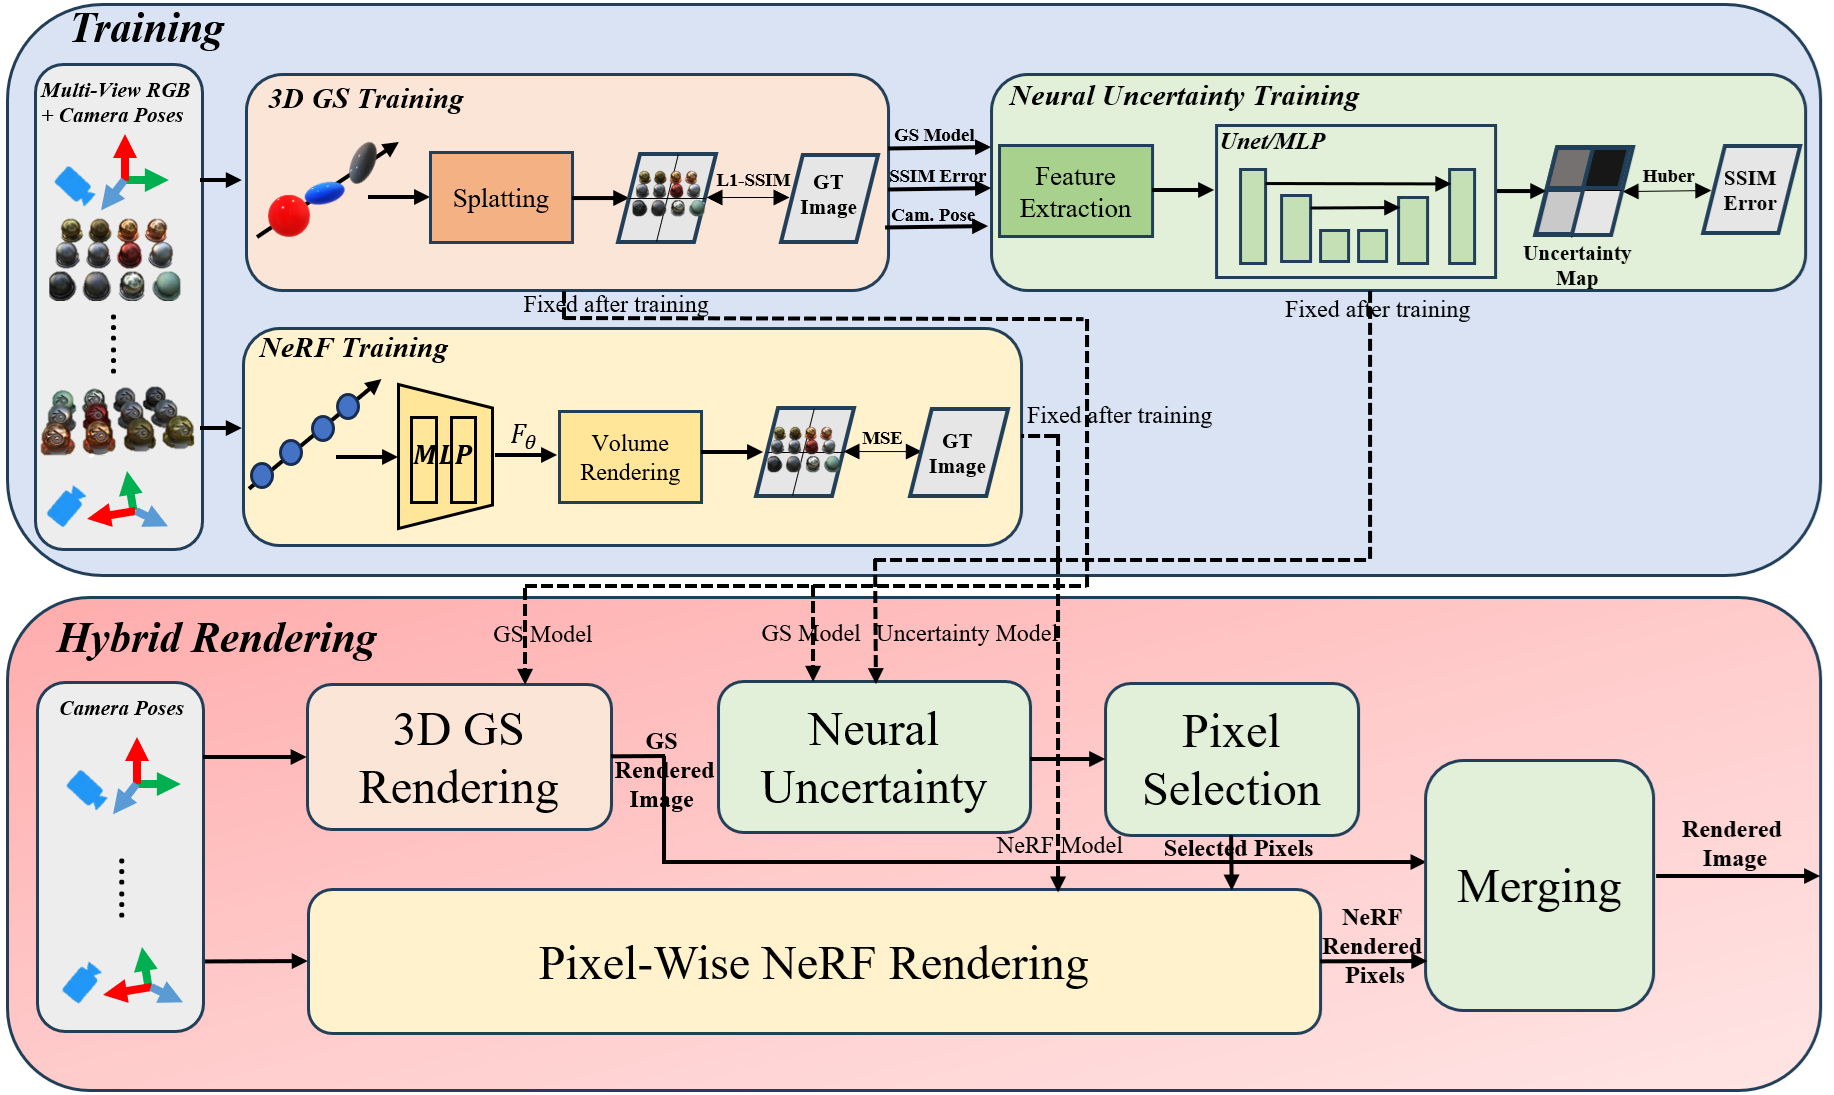
\includegraphics[width=0.9\linewidth]{../Figures/Proposed_Uncertainty_Framework.png}
	\caption{Proposed Uncertainty-Aware Hybrid Rendering Framework.}
	\label{fig:framework}
\end{figure}

We propose an uncertainty-aware hybrid rendering framework that leverages the speed of 3D Gaussian Splatting (GS) and the fidelity of NeRF through uncertainty-guided pixel-wise refinement.  
As shown in Figure~\ref{fig:framework}, the framework consists of three stages:

\vspace{0.3cm}

\subsection{Training Phase}
\textbf{(1) 3D GS Training:} A GS model is trained on multi-view RGB images and camera poses to enable efficient rendering and produce auxiliary features for uncertainty prediction. The training minimizes a perceptual loss that combines L1 and SSIM losses:
\[
\mathcal{L}_{\text{GS}} = \|I_{\text{pred}} - I_{\text{gt}}\|_1 + \lambda_{\text{SSIM}} (1 - \text{SSIM}(I_{\text{pred}}, I_{\text{gt}})),
\]
where $\lambda_{\text{SSIM}}$ is a learnable weight and SSIM is computed over RGB channels.

\textbf{(2) NeRF Training:} A NeRF model is trained independently using the same inputs to generate high-fidelity volume renderings. The loss combines coarse and fine-level MSE losses:
\[
\mathcal{L}_{\text{NeRF}} = 
\begin{cases}
	\text{MSE}(I_{\text{coarse}}, I_{\text{gt}}), & \text{if } \text{epoch} < 100 \\
	\alpha \cdot \text{MSE}(I_{\text{coarse}}, I_{\text{gt}}) + (1 - \alpha) \cdot \text{MSE}(I_{\text{fine}}, I_{\text{gt}}), & \text{otherwise}
\end{cases}
\]
with $\alpha = \max(0.9 - \frac{\text{epoch} - 100}{\text{num\_epochs} - 100}, 0.5)$ to gradually introduce fine supervision.

\textbf{(3) Uncertainty Model Training:} A lightweight U-Net or MLP is trained to predict per-pixel SSIM error from GS-rendered outputs. It uses four GS-derived features (alpha sum, color variance, view direction, 2D covariance area) and camera poses to produce a per-pixel uncertainty map. The training minimizes the smooth L1 (Huber) loss:
\[
\mathcal{L}_{\text{uncertainty}} = \text{Huber}(u_{\text{pred}}, u_{\text{target}}),
\]
where $u_{\text{target}}$ is the SSIM error map and $u_{\text{pred}}$ is the model's prediction.


\subsection{Inference Phase}
\textbf{Input:} A camera pose is provided at test time.

\textbf{Steps:}
\begin{enumerate}[leftmargin=*]
	\item \textbf{GS Rendering:} The GS model renders the full image and extracts feature maps.
	\item \textbf{Uncertainty Prediction:} The uncertainty model predicts per-pixel uncertainty from the GS features.
	\item \textbf{Pixel Selection:} The top-$k$\% most uncertain pixels are selected.
	\item \textbf{NeRF Refinement:} Only the selected pixels are re-rendered using NeRF.
\end{enumerate}

\vspace{1mm}
This hybrid system combines GS rendering with selective NeRF refinement for uncertain pixels, preserving efficiency while enhancing visual quality where needed.

\section{Neural Uncertainty Feature}

\begin{figure}[H]
	\centering
	\includegraphics[width=0.8\linewidth]{../Figures/feature_extraction.png}
	\caption{Feature Extraction for Neural Uncertainty Prediction.}
	\label{fig:uncertainty_feature}
\end{figure}

We extract four types of features from the GS model for uncertainty prediction.  
The input to the feature extraction consists of the output from the trained 3D Gaussian Splatting (GS) model, which includes the parameters of each 3D splat: 3D mean position, orientation quaternion, opacity (alpha), scales (radii), and RGB color values. These attributes are processed together with the known camera pose to generate per-pixel feature maps over the rendered image plane. To be more specific, a 2D Gaussian is represented by the following expression:

\begin{equation}
	f(x; \mu, \Sigma) = \frac{1}{2\pi\sqrt{|\Sigma|}} \exp\left( -\frac{1}{2} (x-\mu)^T \Sigma^{-1} (x-\mu) \right)
\end{equation}

where:
\begin{itemize}
	\item \( x \) is a 2D vector that represents the pixel location
	\item \( \mu \) is the 2D vector representing the mean of the \(i\)-th 2D Gaussian
	\item \( \Sigma \) is the covariance of the 2D Gaussian
\end{itemize}

Given the opacity \(\alpha_i\) of a 3D Gaussian, the alpha value at pixel \(x\) is computed as:

\begin{equation}
	\alpha_i(x) = \alpha_i \exp(P(x,i))
\end{equation}

where

\begin{equation}
	P(x,i) = -\frac{1}{2} (x-\mu)^T \Sigma^{-1} (x-\mu)
\end{equation}

Thus, \(\alpha_i(x)\) represents the contribution of the \(i\)-th Gaussian to the pixel opacity at location \(x\).

We extract four pixel-wise features from the GS model for uncertainty prediction:

\begin{itemize}
	\item \textbf{Alpha sum:} Measures total accumulated opacity per pixel:
	\begin{equation}
		\text{Alpha Sum}(x, y) = \sum_{i=1}^{N} \alpha_i(x, y)
	\end{equation}
	It indicates overall visibility, helping detect under-/over-blended regions with high uncertainty.
	
	\item \textbf{Color variance:} Reflects RGB variance of splats using opacity-weighted transmittance:
	\begin{equation}
		\text{Color Variance}(x, y) = \frac{1}{3} \sum_{c \in \{R,G,B\}} \frac{\sum_{i=1}^{N} w_i(x,y) (c_i(x,y) - \bar{c}(x,y))^2}{\sum_{i=1}^{N} w_i(x,y)}
	\end{equation}
	where $w_i(x,y) = \alpha_i(x,y) \times \text{transmittance}_i(x,y)$ and $\bar{c}(x,y)$ is the weighted mean color:
	\begin{equation}
		\bar{c}(x, y) = \frac{\sum_{i=1}^{N} w_i(x,y) c_i(x,y)}{\sum_{i=1}^{N} w_i(x,y)}
	\end{equation}
	Higher color variance suggests texture discontinuities or occlusion boundaries.
	
	\item \textbf{2D covariance area:} Represents projected splat size:
	\begin{equation}
		\text{Covariance Area}(x, y) = \frac{\sum_{i=1}^{N} \alpha_i(x, y) \cdot \text{det}(\Sigma_i)}{\sum_{i=1}^{N} \alpha_i(x, y)}
	\end{equation}
	Larger splats often correlate with depth ambiguity or blending, signaling higher uncertainty.
	
	\item \textbf{View direction cosine:} Measures alignment between viewing direction and splat normal:
	\begin{equation}
		\cos\theta(x, y) = \frac{\sum_{i=1}^{N} \alpha_i(x, y) \cdot \cos(\theta_i)}{\sum_{i=1}^{N} \alpha_i(x, y)}
	\end{equation}
	Oblique angles often imply lower visibility and greater uncertainty.
\end{itemize}

These four maps, each of shape $[H, W]$, are stacked to form a $[H, W, 4]$ tensor, which is input to a neural network (MLP or U-Net) for per-pixel SSIM-based uncertainty prediction.

\section{Experiment Setup}

\subsection{Dataset Introduction}
We use the NeRF Synthetic Dataset, which consists of photorealistic scenes rendered from synthetic 3D assets. It provides multi-view RGB images and ground-truth camera poses for each scene. Both the training and validation sets contain 100 images and correspondent camera poses each, while the test set includes 200 images and camera poses. Our experiments focus on the “materials” scene.

\subsection{Environment and Hyperparameter Setting}
Our experiments run on an NVIDIA GPU (CUDA 12.7, driver 565.57.01) with Python 3.10, PyTorch, and standard deep learning libraries on Linux.

For Gaussian Splatting (GS), we use 15,000 3D points, 128×128 resolution, and SSIM-based supervision. The MLP model is trained for 101 epochs (LR = $4 \times 10^{-3}$), and the U-Net model for 201 epochs (LR = $1 \times 10^{-3}$). NeRF is trained for 3001 epochs with batch size 512, using coarse-to-fine sampling (512 pts/ray: 256 coarse + 150 fine), LR = $1 \times 10^{-4}$ with decay (×0.7 every 50 epochs). Input images are 128×128 with 10 harmonic encodings for position and 3 for view direction, using an 8-layer MLP. During inference, hybrid rendering applies NeRF only to the top 5\%–50\% most uncertain pixels.



\section{Qualitative Result}
 The input to our framework includes multi-view images and camera poses, and the output is a high-quality novel view synthesized using a hybrid rendering pipeline that combines 3D Gaussian Splatting and pixel-wise NeRF refinement based on uncertainty prediction. We compare a lightweight 1K-parameter two-layer MLP (Spearman: 0.756) and a 110K-parameter U-Net (Spearman: 0.890) for uncertainty modeling.
 
 For full 360° reconstruction visualizations, please visit our project webpage: \url{https://www.andrew.cmu.edu/course/16-825/projects/bochunc/final_proj/}.
 
 
\subsection{Implemented Uncertainty Prediction Model: U-Net}
The following Table~\ref{tab:Hyb-UNetRender} presents the hybrid rendering results using U-Net with 110K parameters for uncertainty prediction, where the top ( k\% ) of pixels with the highest uncertainty are re-rendered using pixel-wise NeRF refinement.

\begin{table}[H]
	\centering
	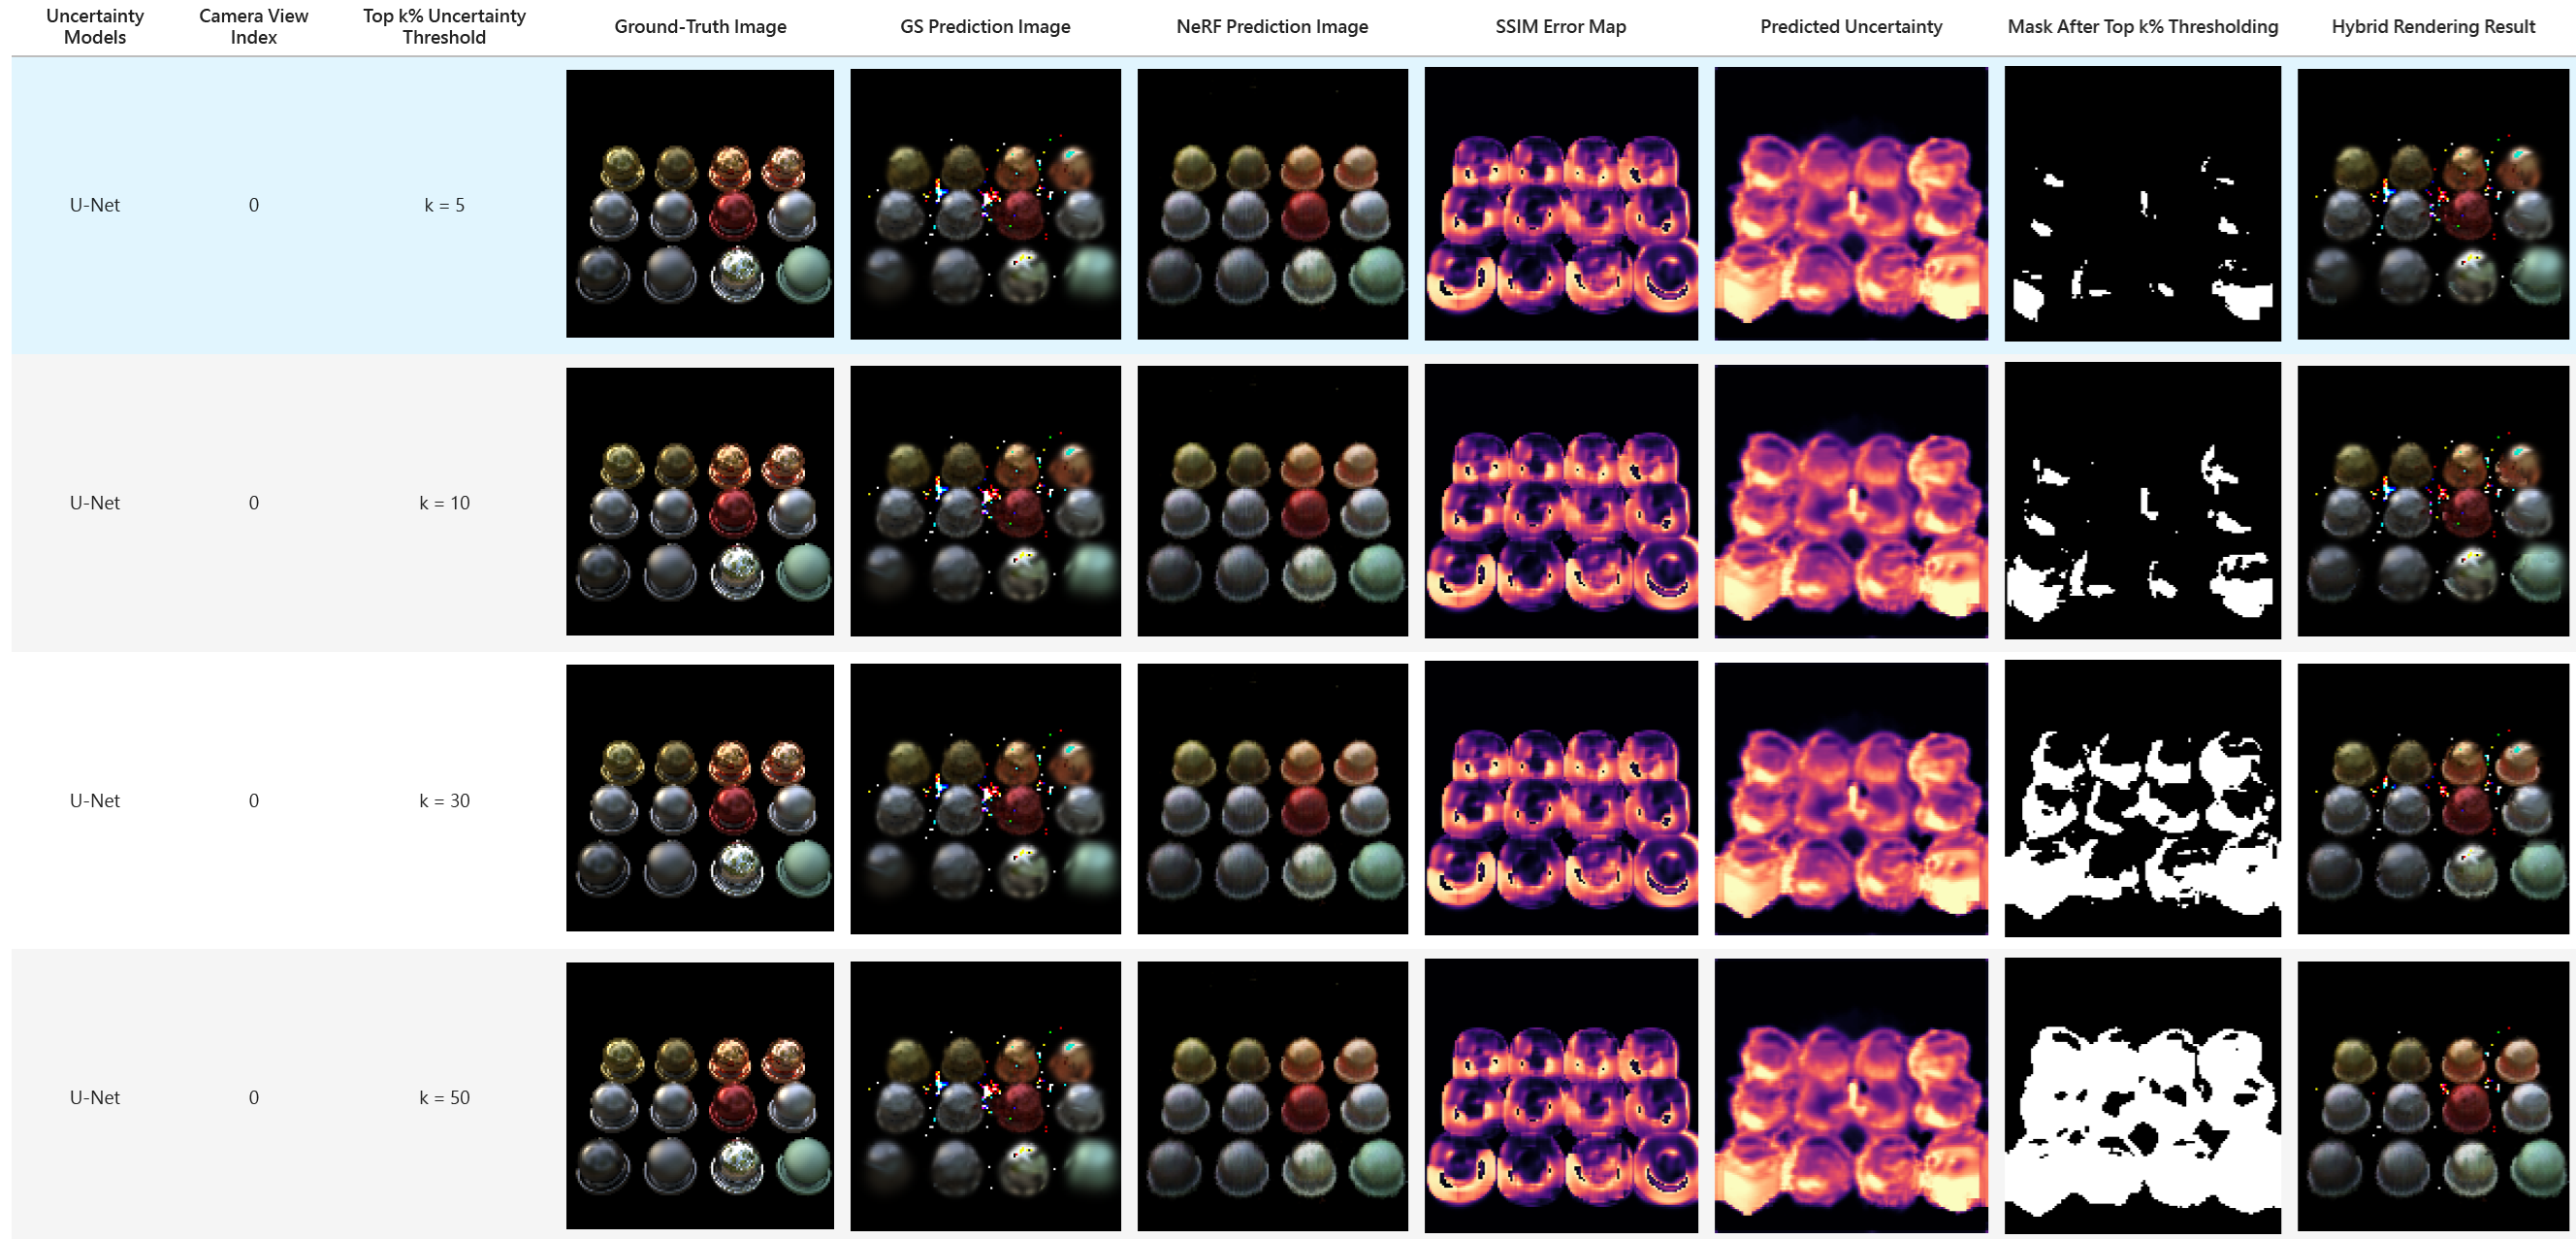
\includegraphics[width=0.8\linewidth]{../Figures/unet_cmp.png}
	\caption{Hybrid-UNet Rendering Results Under Different k Values.}
	\label{tab:Hyb-UNetRender}
\end{table}

We observe that with $k = 30$ or $k = 50$, hybrid rendering achieves fidelity close to full NeRF rendering. As $k$ increases, more uncertain regions are refined by NeRF, improving perceptual quality. When $k = 5$ or $k = 10$, limited refinement leads to visible quality gaps. However, at higher $k$ values, important structures are corrected while simpler regions remain efficiently rendered by Gaussian Splatting. This confirms that uncertainty-guided hybrid rendering balances fidelity and efficiency by selectively applying NeRF only where needed.


\subsection{Implemented Uncertainty Prediction Model: MLP}

The following Table~\ref{tab:Hyb-MLPRender} changes the uncertainty prediction model from a 110K-parameter U-Net to a simple two-layer MLP with only 1K parameters. We can further compare Table~\ref{tab:Hyb-MLPRender} and Table~\ref{tab:Hyb-UNetRender} to evaluate whether the complexity of the uncertainty prediction model is necessary for hybrid rendering fidelity.


\begin{table}[H]
	\centering
	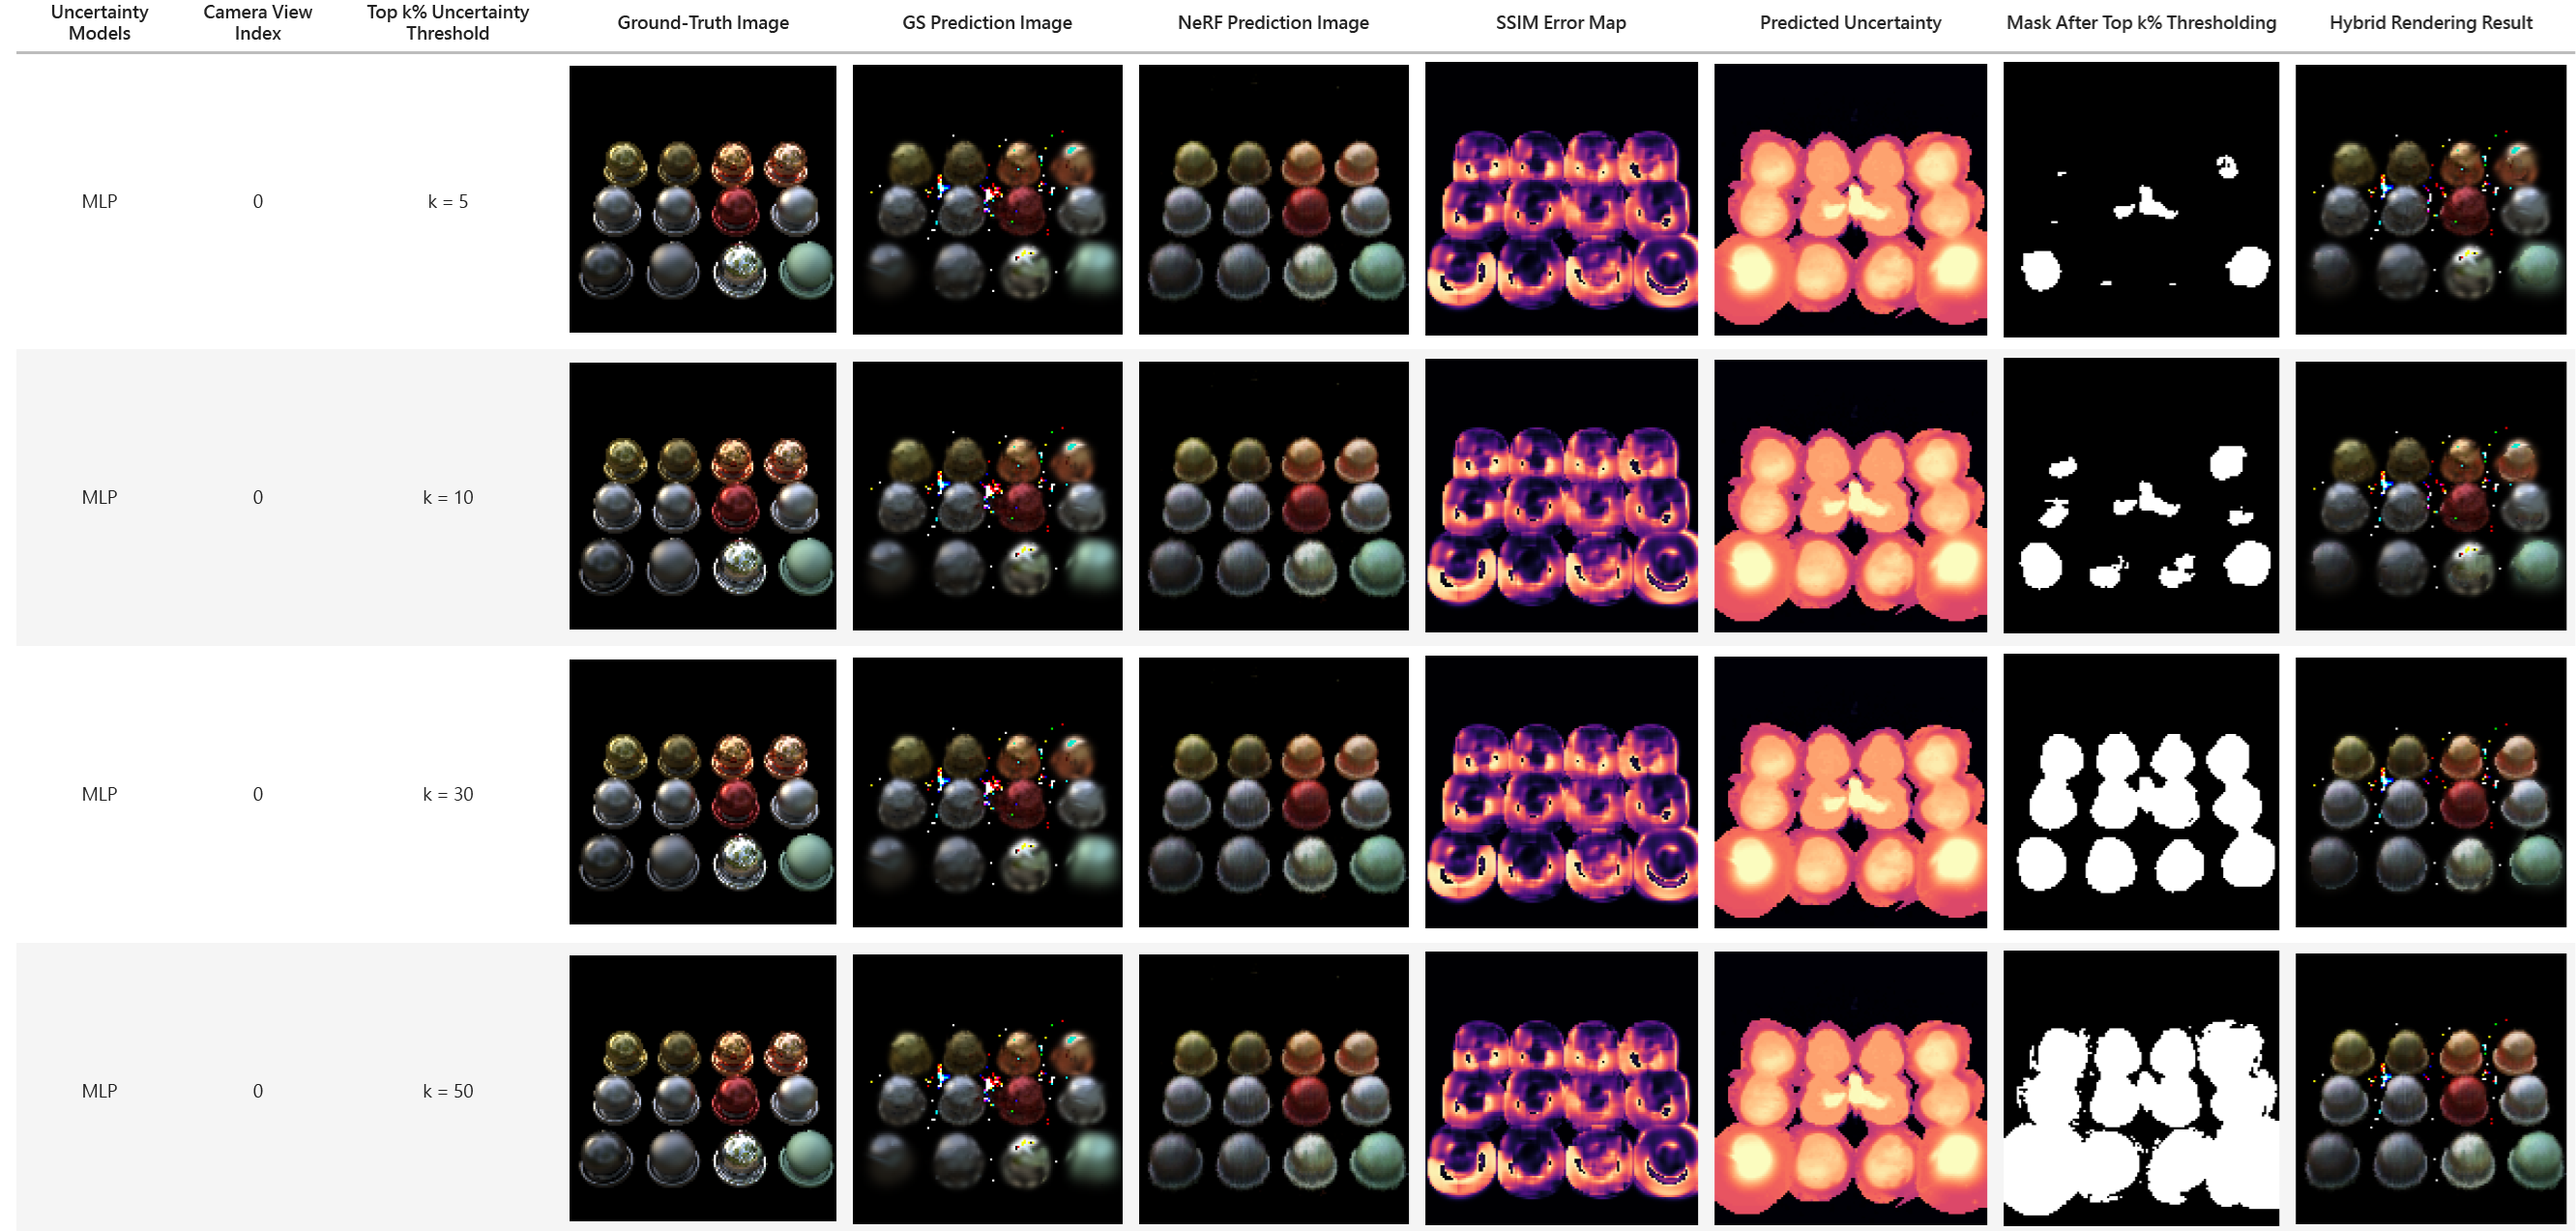
\includegraphics[width=0.8\linewidth]{../Figures/mlp_cmp.png}
	\caption{Hybrid-MLP Rendering Results Under Different k Values.}
	\label{tab:Hyb-MLPRender}
\end{table}

From above tables, we observe that an MLP-based uncertainty predictor yields hybrid renderings with comparable fidelity to U-Net when using higher top-$k\%$ thresholds ($k=30$ or $50$). While $k=5$ or $10$ results in visible quality gaps due to limited NeRF refinement, higher thresholds enable recovery of high-frequency details. This shows that even a lightweight MLP can effectively guide selective NeRF refinement, maintaining perceptual quality while preserving GS efficiency.


\subsection{More Rendering Results Using These Two Models Under Different Camera Views}
As $k = 30$ could provide high fidelity results, we further view the hybrid rendering results with $k = 30$ under different camera views (by changing the camera view index in the test dataset). The following Table~\ref{tab:Hyb-viewsRender} shows the results.

\begin{table}[H]
	\centering
	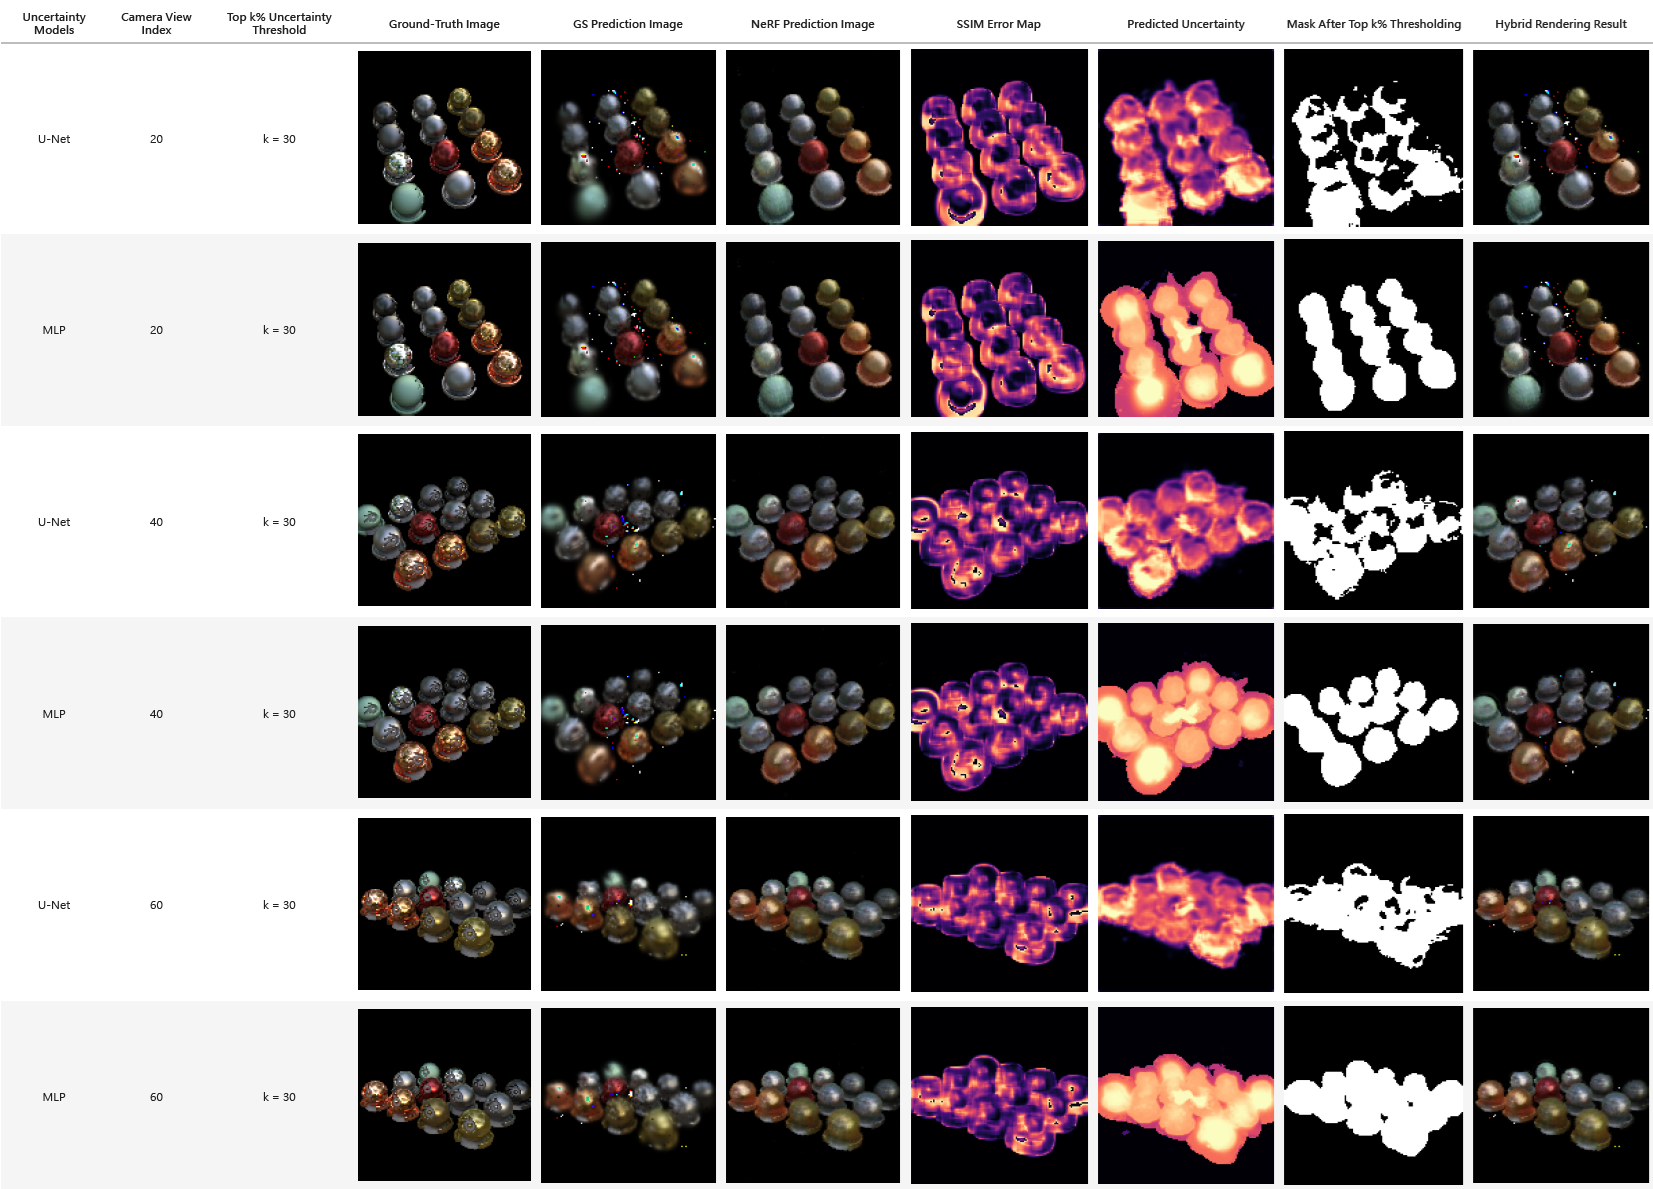
\includegraphics[width=0.8\linewidth]{../Figures/views_cmp.png}
	\caption{Hybrid Rendering Results of the Two Models Under Different Camera Views.}
	\label{tab:Hyb-viewsRender}
\end{table}

Across different camera views, hybrid rendering with ($k = 30$) consistently achieves high perceptual quality. Both U-Net and MLP-based models effectively identify uncertain regions for NeRF refinement. Despite the MLP’s lower parameter count, its results are comparable to U-Net’s. This shows our uncertainty-aware hybrid framework is robust to viewpoint changes and that lightweight models can maintain high rendering fidelity.

\section{Quantitative Results}

The following Table~\ref{tab:Res} summarizes the rendering quality and runtime results with Gaussian Splatting method only (GS only), NeRF method only (NeRF only), SS Mip-NeRF method, and our hybrid rendering method at different replacement rates with MLP and U-Net models for uncertainty prediction:

\begin{table}[H]
	\centering
	\scriptsize
	\begin{tabular}{|l|c|c|c|c|c|c|}
		\hline
		Method & PSNR $\uparrow$ & SSIM $\uparrow$ & GS Time (s) & NeRF Time (s) & Total Time (s) & Replace \% \\
		\hline
		GS only         & 22.23 & 0.819 & 0.246 & - & 0.246 & 0\% \\
		NeRF only       & 24.76 & 0.891 & - & 0.827 & 0.827 & 100\% \\
		SS Mip-NeRF     & \textbf{32.60} & - & - & 0.864 & 0.864 & 100\% \\
		Hybrid-MLP 5\%  & 22.39 & 0.824 & 0.272 & 0.040 & 0.312 & \textasciitilde 5\% \\
		Hybrid-MLP 10\% & 22.64 & 0.832 & 0.272 & 0.081 & 0.353 & \textasciitilde 10\% \\
		Hybrid-MLP 30\% & 24.31 & 0.875 & 0.272 & 0.220 & 0.492 & \textasciitilde 30\% \\
		\textbf{Hybrid-MLP 50\%} & 24.75 & \textbf{0.892} & 0.271 & 0.397 & \textbf{0.668} & \textasciitilde 50\% \\
		Hybrid-UNet 5\% & 22.58 & 0.836 & 0.275 & 0.040 & 0.315 & \textasciitilde 5\% \\
		Hybrid-UNet 10\% & 22.88 & 0.847 & 0.274 & 0.079 & 0.353 & \textasciitilde 10\% \\
		Hybrid-UNet 30\% & 24.11 & 0.880 & 0.274 & 0.220 & 0.494 & \textasciitilde 30\% \\
		\textbf{Hybrid-UNet 50\%} & 24.73 & \textbf{0.892} & 0.274 & 0.399 & \textbf{0.673} & \textasciitilde 50\% \\
		\hline
	\end{tabular}
	\caption{Rendering Quality and Runtime Comparison Under Different Replacement Ratios.}
	\label{tab:Res}
\end{table}

\noindent \textbf{Note:}
\begin{itemize}
	\item GS Time refers to the time spent on feature extraction using the GS model.
	\item NeRF Time refers to the time spent on ray-marching and rendering using NeRF for selected pixels.
\end{itemize}

As shown in Table~\ref{tab:Res}, our hybrid method achieves higher SSIM scores (up to \textbf{0.892}) and comparable PSNR values (up to \textbf{24.75}) compared to both the GS-only (PSNR: \textbf{22.23}, SSIM: \textbf{0.819}) and NeRF-only (PSNR: \textbf{24.76}, SSIM: \textbf{0.891}) baselines. Notably, the \textbf{Hybrid-MLP 50\%} model not only matches the perceptual quality of NeRF but also reduces the total rendering time to \textbf{0.668s}, significantly faster than NeRF-only (\textbf{0.827s}) and the state-of-the-art SS Mip-NeRF (\textbf{0.864s}) while maintaining only a modest increase over GS-only (\textbf{0.246s}). The \textbf{Hybrid-UNet 50\%} model has comparable perceptual quality and speed that only takes \textbf{0.673s}, only 0.005s more than \textbf{Hybrid-MLP 50\%} model, to finish a frame. This demonstrates that our hybrid approach can deliver superior visual fidelity at a fraction of the computational cost.


We further analyze the feature extraction cost with $k=50$ (Replace 50\%) as the following tables:

\subsection*{Profiling for Hybrid-UNet Feature Extraction}
\begin{table}[H]
	\centering
	\scriptsize
	\begin{tabular}{|l|c|c|}
		\hline
		Step & Time (s) & Percentage \\
		\hline
		Whole feature extraction   & 0.2740 & 100\% \\
		Compute alpha sum          & 0.2180 & 79.56\% \\
		Compute color variance     & 0.0350 & 12.77\% \\
		Compute 2D covariance (proj\_gau)      & 0.0080 & 2.92\% \\
		Compute 2D covariance area (footprint\_area) & 0.0040 & 1.46\% \\
		Compute view direction     & 0.0034 & 1.24\% \\
		Model feed-forward         & 0.0033 & 1.20\% \\
	    Compute depth and sorting  & 0.0010 & 0.36\% \\
	    Select top-$k$ and mask    & 0.0009 & 0.34\% \\
	    Flatten                    & 0.0004 & 0.15\% \\
		\hline
	\end{tabular}
	\caption{Hybrid-UNet Feature Extraction Breakdown at $k=50$.}
\end{table}

\subsection*{Profiling for Hybrid-MLP Feature Extraction}
\begin{table}[H]
	\centering
	\scriptsize
	\begin{tabular}{|l|c|c|}
		\hline
		Step & Time (s) & Percentage \\
		\hline
		Whole feature extraction   & 0.2710 & 100\% \\
		Compute alpha sum          & 0.2170 & 80.07\% \\
		Compute color variance     & 0.0350 & 12.92\% \\
		Compute 2D covariance (proj\_gau)      & 0.0080 & 2.95\% \\
		Compute 2D covariance area (footprint\_area) & 0.0040 & 1.48\% \\
		Compute view direction     & 0.0034 & 1.25\% \\
		Model feed-forward         & 0.0013 & 0.48\% \\
		Compute depth and sorting  & 0.0010 & 0.37\% \\
		Select top-$k$ and mask    & 0.0009 & 0.33\% \\
		Flatten                    & 0.0004 & 0.15\% \\
		\hline
	\end{tabular}
	\caption{Hybrid-MLP Feature Extraction Breakdown at $k=50$.}
\end{table}

\noindent We profile the feature extraction process for both Hybrid-UNet and Hybrid-MLP. Most of the time is spent on \textbf{alpha sum computation} ($\sim$80\%) and \textbf{color variance} ($\sim$13\%), with all other steps contributing less than 3\%.

Hybrid-MLP is slightly faster overall (0.2710s vs. 0.2740s) due to its smaller model and faster inference (0.0013s vs. 0.0033s). Despite this, both models share nearly identical time breakdowns, indicating that the main bottleneck lies in \textbf{feature computation} (especially alpha sum), not model complexity.



	
	\bibliographystyle{plain}
	\begin{thebibliography}{9}
		\bibitem{mildenhall2020nerf} B. Mildenhall, P. P. Srinivasan, M. Tancik, et al. NeRF: Representing Scenes as Neural Radiance Fields for View Synthesis. ECCV 2020.
		\bibitem{kerbl2023gaussians} B. Kerbl, G. Kopanas, T. Leimkühler, and G. Drettakis. 3D Gaussian Splatting for Real-Time Radiance Field Rendering. *ACM Transactions on Graphics*, vol. 42, no. 4, Jul. 2023. Available: \url{https://repo-sam.inria.fr/fungraph/3d-gaussian-splatting/}.		
		\bibitem{barron2021mipnerf} J. Barron, B. Mildenhall, et al. Mip-NeRF: A Multiscale Representation for Anti-Aliasing Neural Radiance Fields. ICCV 2021.
		
		%\bibitem{reizenstein2021co3d} J. Reizenstein, R. Shapovalov, et al. Common Objects in 3D: Large-Scale Learning and Evaluation of Real-life 3D Category Reconstruction. ICCV 2021.
		%\bibitem{dai2017scannet} A. Dai, A. X. Chang, et al. ScanNet: Richly-annotated 3D Reconstructions of Indoor Scenes. CVPR 2017.
		%\bibitem{knapitsch2017tanks} A. Knapitsch, J. Park, et al. Tanks and Temples: Benchmarking Large-Scale Scene Reconstruction. CVPR 2017.	
	\end{thebibliography}
	
\end{document}